\documentclass[10pt,a4paper]{ctexart}
\usepackage[margin=2cm]{geometry}
\usepackage{graphicx}
\usepackage{float}      % 支持 [H] 浮动体选项
\usepackage{hyperref}
\usepackage{amsmath}    % 提供方程环境
\usepackage{physics}    % 简化向量、微分算子语法
\newcommand{\myspace}[1]{\par\vspace{#1\baselineskip}} %自定义空一行
\usepackage{fancyhdr}
\usepackage{tabularx}
\pagestyle{fancy}
\fancyhf{}  % 清除所有页眉页脚
\fancyfoot[C]{\thepage}  % 在页脚中央设置页码
\renewcommand{\headrulewidth}{0pt}  % 去掉页眉横线
\renewcommand{\footrulewidth}{0pt}  % 去掉页脚横线

\usepackage{hyperref}
\hypersetup{
    colorlinks=true,
    linkcolor=blue,
    filecolor=magenta,      
    urlcolor=cyan,
    pdftitle={Overleaf Example},
    pdfpagemode=FullScreen,
    }

\usepackage{titlesec}

% 重新定义section格式
\titleformat{\section}
  {\normalfont\Large\bfseries}
  {\chinese{section}、}
  {0pt}
  {}

% 给出常用字号的自定义指令
\newcommand{\chuhao}{\fontsize{42pt}{48pt}\selectfont}
\newcommand{\xiaochu}{\fontsize{36pt}{42pt}\selectfont}
\newcommand{\xiaoer}{\fontsize{18pt}{21.6pt}\selectfont}
\newcommand{\sanhao}{\fontsize{16pt}{20pt}\selectfont}
\newcommand{\xiaosan}{\fontsize{15pt}{18pt}\selectfont}
\newcommand{\sihao}{\fontsize{14pt}{18pt}\selectfont}
\newcommand{\xiaosi}{\fontsize{12pt}{16pt}\selectfont}
\newcommand{\wuhao}{\fontsize{10.5pt}{12.6pt}\selectfont}

% 定义中文数字转换
\titleformat{\section}
  {\normalfont\Large\bfseries}
  {\zhnum{section}、}  % 使用\zhnum而不是\chinese
  {0pt}
  {}

% 标题设置
\title{\xiaochu\textbf{物理实验报告}}
\author{}
\date{}

\begin{document}

\vspace*{36pt} % 顶部空白

% 居中填写区域
\begin{center}
    
\includegraphics[width = 9cm]{figure/head.png}
    
    \xiaochu\textbf{物理实验报告}
    % 预留空白区域
    \vspace{13pt}
    \vspace{13pt}
    \vspace{13pt}
    \vspace{13pt}
    
    \sanhao\textbf{实验名称：\underline{\makebox[10cm]{ 用双臂电桥测低电阻}}} \\[10pt]
    \sanhao\textbf{实验桌号：\underline{\makebox[10cm]{ 3}}} \\[10pt]
    \sanhao\textbf{指导教师：\underline{\makebox[10cm]{ 刘公羽 }}} \\[30pt]
    
    % 预留空白区域
    \myspace{6}
    
   \sihao\textbf{班级：\underline{\makebox[6cm]{}}} \\[10pt]
    \sihao\textbf{姓名：\underline{\makebox[6cm]{}}} \\[10pt]
    \sihao\textbf{学号：\underline{\makebox[6cm]{}}} \\[30pt]
    
   \sihao\textbf{实验日期: 
   \underline{\makebox[0.8cm]{2025}}  年 
   \underline{\makebox[0.4cm]{12}}月
   \underline{\makebox[0.4cm]{17}}日  
   星期\underline{\makebox[0.6cm]{三}}上午}
    
    \vspace{18pt}
    \sihao 浙江大学物理实验教学中心
    
\end{center}

\newpage

\section{预习报告}

    \subsection{实验综述}
    
    \xiaosi （自述实验现象、实验原理和实验方法，不超过300字，5分）

     r1和r2代表接触电阻和导线电阻，一般在0.01-1 Ω的数量级。
    由图可见，当测量电阻时r1和r2会包含于内，实际测得的阻值为Rx+r1+r2，当Rx与r1、r2同数量级时引入的误差就很大。
\begin{figure}[H]
        \centering
        
\includegraphics[width=0.8\textwidth]{figure/circuit.png}
        \caption{接触电阻影响示意图}
    \end{figure}

    因此发明了双臂电桥测电阻的办法。等效电路如图
    \begin{figure}[H]
        \centering
        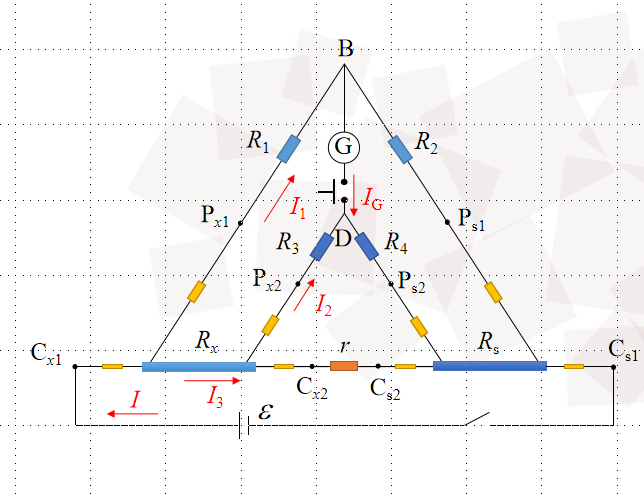
\includegraphics[width=0.8\textwidth]{figure/bridge.png}
        \caption{双臂电桥电路图}
    \end{figure}
    根据基尔霍夫定律可以得到，在$\frac{R_1}{R_2}=\frac{R_3}{R_4}$时$R_x=\frac{R_1}{R_2}R_s$

    室温下温度变化不大时金属温阻表现为线性$R_t=R_0(1+\alpha t)$。

    利用双臂电桥法测量电阻，改变温度，就可以绘制金属电阻-温度曲线，测量温度系数。
    \myspace{2}
    
    
    \subsection{实验重点}
    
    \xiaosi（简述本实验的学习重点，不超过100字，3分）
    
掌握双臂电桥测量低电阻的原理和使用方法

了解单臂电桥与双臂电桥的关系和区别
    \myspace{2}
    
    \subsection{实验难点}
    
    \xiaosi（简述本实验的实现难点，不超过100字，2分）

    准确控制温度。温度不易控制，且达到设定温度后会有惯性或者冷却，需要迅速完成对应的实验操作。

    准确测量金属电阻的直径、长度等参数。
\myspace{2}
\section{原始数据}

    \xiaosi （将有老师签名的“自备数据记录草稿纸”的扫描或手机拍摄图粘贴在下方，20分）
   
\begin{figure}[H]
    \centering
    
\includegraphics[width=0.8\textwidth]{figure/raw_data.jpg}
    \caption{原始数据记录}
    \label{fig:raw_data}
\end{figure}
\section{结果与分析}

    \subsection{数据处理与结果}
    \xiaosi （列出数据表格、选择数据处理方法、给定测量或计算结果，30分）

    \subsubsection{测量金属导体电阻率}
    实验首先测量金属阻值、直径、长度，计算电阻率。

   \begin{table}[H]
\centering
\caption{电阻率相关参数测量数据记录表}
\label{tab:magnetic_field}
\begin{tabular}{|c|c|c|}
\hline
$R(\Omega)$ & $d(\text{mm})$ & $L(\text{cm})$ \\
\hline
$5.614 \times 10^{-4}$ & 4.32 & 25.01 \\
\hline
\end{tabular}
\end{table}
计算电阻率平均值$\bar{\rho}=\frac{\pi \bar R \bar d^2}{4 \bar L}=3.29 \times 10^{-8} \Omega \cdot \text{m}$。

不确定计算需要使用传递公式。
\[
u(R)=\frac{9.999 \times 10^{-4} \times 0.2\%}{\sqrt{3}}=1.154 \times 10^{-6} \Omega
\]
\[
u(d)=\frac{0.02}{\sqrt{3}}=0.0115 \text{mm}
\]
\[
u(L)=\frac{0.05}{\sqrt{3}}=0.0289 \text{cm}
\]
\[
\frac{u(\rho)}{\rho}=\sqrt{\left(\frac{u(R)}{R}\right)^2+\left(2\frac{u(d)}{d}\right)^2+\left(\frac{u(L)}{L}\right)^2}=3.556 \times 10^{-3} \Omega \cdot \text{m}
\]
\[
u(\rho)=1.2 \times 10^{-10} \Omega \cdot \text{m}
\]
最终结果为$\rho=(3.290 \pm 0.012) \times 10^{-8} \Omega \cdot \text{m}$
\subsubsection{测量金属导体电阻温度系数}

利用直流双臂电桥在不同温度下测量金属阻值。数据如下：
\begin{table}[H]
\centering
\caption{直流双臂电桥测温度特性数据记录表}
\vspace{2mm}
{\small \centering 实验条件： \quad $\alpha_{\mathrm{theory}}=4.33 \times 10^{-3} /^{\circ}\mathrm{C}$ \par}
\vspace{2mm}
\begin{tabularx}{0.9\textwidth}{>{\centering\arraybackslash}p{0.2\textwidth}|*{10}{>{\centering\arraybackslash}X}}
\hline
次序 & 1 & 2 & 3 & 4 & 5 & 6 & 7 & 8 & 9 & 10\\
\hline
温度 $t/^{\circ}\mathrm{C}$ &14.3 &21.5 &25.4 &30.7 &35.1 &41.2 &45.1 &50.0 & 55.2 & 60.0 \\
\hline
$R_t/10^{-3}\Omega$ & 4.563&4.675 &4.740 &4.843 &4.920 &5.019 &5.113 &5.191&5.295&5.375 \\
\hline
\end{tabularx}
\end{table}


根据公式 $\alpha_t = \frac{R_{x(t+5)}-R_{xt}}{R_{xt}t_{t+5} - R_{x(t+5)}t_t}$ 利用逐差法计算温度系数，得到下方表格

\begin{table}[H]
\centering
\caption{逐差法计算得到的电阻温度系数 $\alpha$}
\vspace{2mm}
\begin{tabular}{|c|c|}
\hline
组次  & $\alpha_i/10^{-3} \,^{\circ}\mathrm{C}^{-1}$ \\ \hline
1 &  3.92 \\ \hline
2 & 4.34 \\ \hline
3 &  4.29 \\ \hline
4 & 4.31 \\ \hline
5 &  4.27 \\ \hline
\end{tabular}
\end{table}

平均值：
\[
\bar{\alpha} = \frac{3.92 + 4.34 + 4.29 + 4.31 + 4.27}{5} \times 10^{-3}
\approx 4.23 \times 10^{-3} \; /^\circ\mathrm{C}
\]

与理论值 $\alpha_{\mathrm{theory}} = 4.33 \times 10^{-3} /^\circ\mathrm{C}$ 的相对误差：
\[
\frac{|4.23 - 4.33|}{4.33} \times 100\% \approx 2.3\%.
\]

另一种方法是利用线性拟合得到温度系数。利用最小二乘法对$R_t$-$t$数据进行线性
拟合$R_t$-$t$图像如下
\begin{figure}[H]
    \centering
    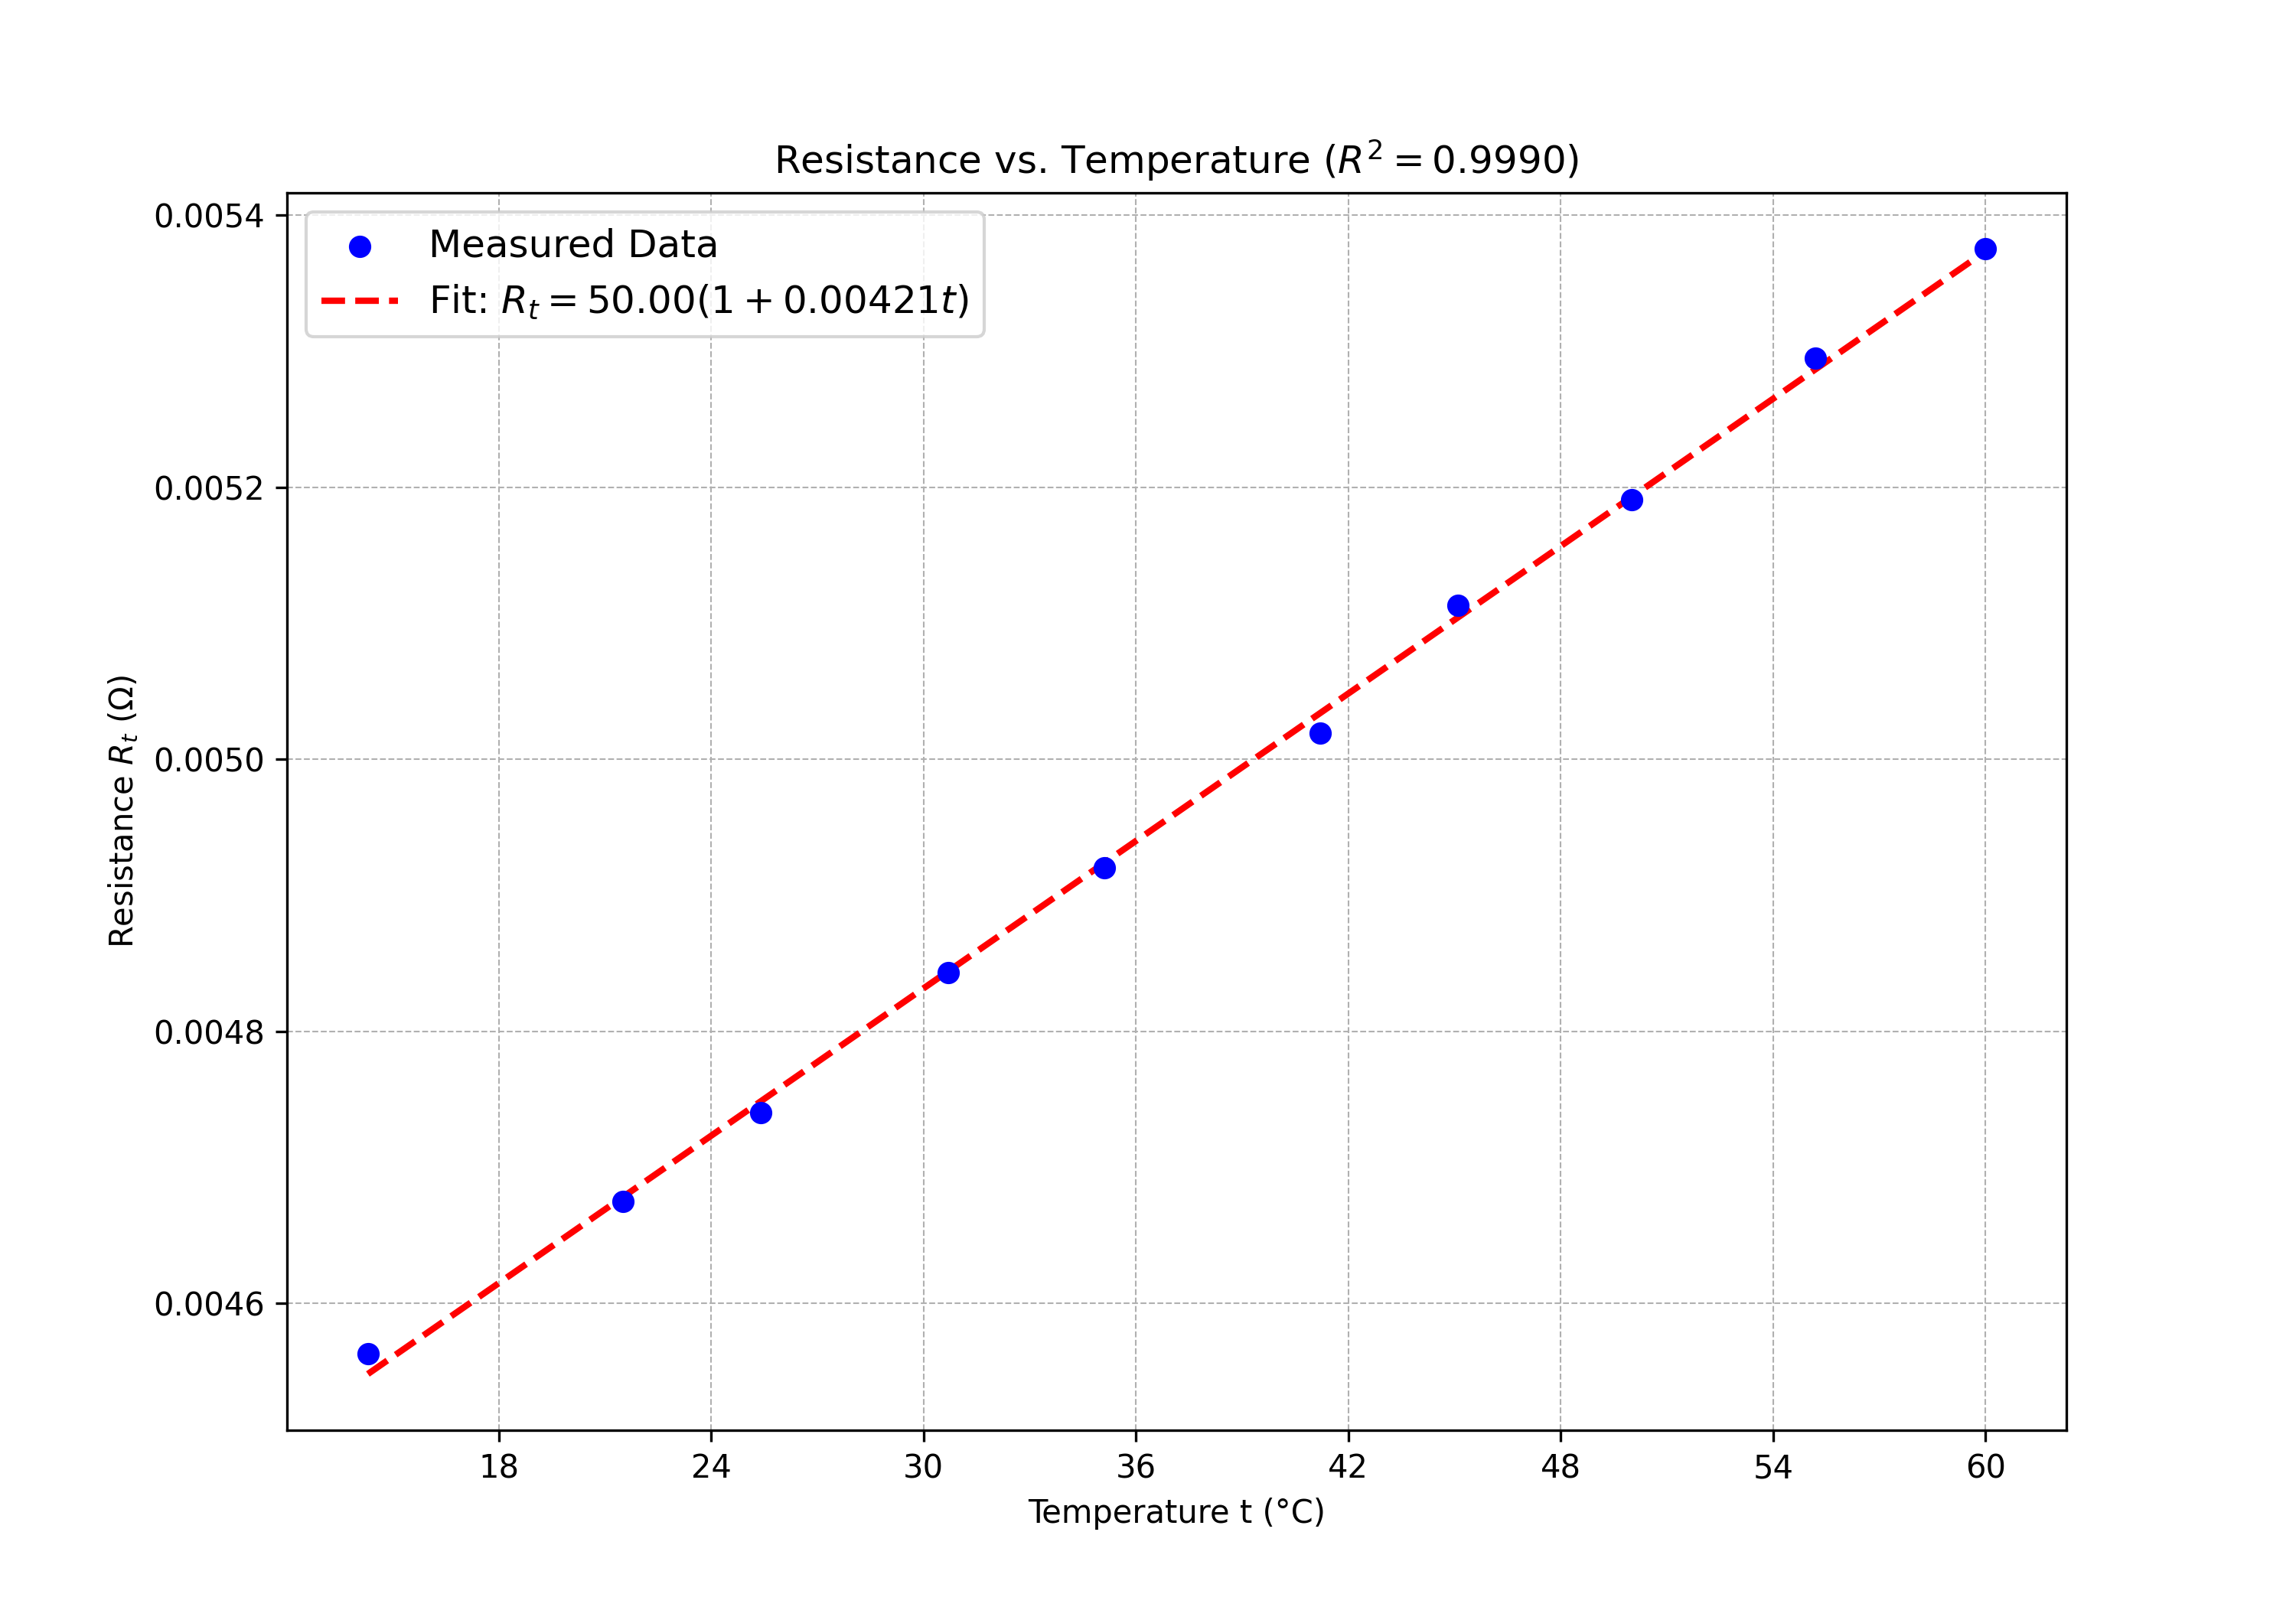
\includegraphics[width=0.8\textwidth]{figure/image.png}
    \caption{电阻-温度拟合曲线}
    \label{fig:fit} 
\end{figure}
得到温度系数$\alpha=4.21 \times 10^{-3} /^{\circ}\mathrm{C}$
拟合优度$R^2=0.9990$，拟合效果较好。
温度系数相对误差为
\[\frac{|\alpha-\alpha_{\mathrm{theory}}|}{\alpha_{\mathrm{theory}}}=2.8\%\]
    \myspace{2}
    \myspace{2}
    \subsection{误差分析}
    \xiaosi （运用测量误差、相对误差、不确定度等分析实验结果，20分）
    
    本实验的误差主要来源于以下几个方面：
    
       \begin{itemize}
           \item \textbf{多次读数波动}：电桥平衡点判断存在主观性，尤其是在接近平衡时，检流计指针的微小摆动可能带来读数偏差。
           \item \textbf{温度控制与读数不同步}：升温过程中设定温度点难以精确停留，且电阻测量与温度读数存在微小时间差，导致数据点$(t, R_t)$并非严格同步。
           \item \textbf{金属棒几何尺寸测量}：直径和长度在不同位置测量结果略有差异。
            \item \textbf{仪器精度限制}：电桥、电压表和温度计的固有精度限制了测量的准确性。
       \end{itemize}
    
    两种方法得到的温度系数与理论值$4.33 \times 10^{-3} /^\circ\mathrm{C}$的相对误差分别为2.3\%和2.8\%，均在可接受的范围内。电阻率测量结果$\rho = (3.290 \pm 0.012) \times 10^{-8} \Omega\cdot\mathrm{m}$。
    综合来看，实验结果与理论值吻合较好，主要误差来源是温度测量的非理想同步性与仪器的固有精度限制。通过更精密的温控设备和更高精度的测量仪器可进一步减小误差。
    
    \myspace{2}
    
    \subsection{实验探讨}
    \xiaosi （对实验内容、现象和过程的小结，不超过100字，10分）
    
    本实验通过双臂电桥法成功测量了低电阻及金属电阻温度系数。
    掌握了双臂电桥消除引线电阻影响的原理和操作方法。
    实验证实金属电阻随温度升高线性增加，通过逐差法和线性拟合得到的温度系数与理论值接近，验证了理论的正确性。
    实验难点在于升温过程的温度控制和同步测量，需操作迅速、配合默契。

\section{思考题}

    \xiaosi （解答教材或讲义或老师布置的思考题，10分）
    
    \begin{enumerate}
        \item \textbf{双臂电桥与惠斯登电桥有哪些异同？}
        
        \textbf{相同点：}
        \begin{itemize}
            \item 两者均基于电桥平衡原理（$\frac{R_1}{R_2}=\frac{R_3}{R_4}$时检流计无电流）。
            \item 基本结构都包含四个桥臂和一个检流计。
        \end{itemize}
        
        \textbf{不同点：}
        \begin{itemize}
            \item \textbf{测量对象}：惠斯登电桥通常测量中值电阻（$10\Omega \sim 1M\Omega$）；双臂电桥专为测量低电阻（$<1\Omega$）设计。
            \item \textbf{结构/端钮}：惠斯登电桥使用二端电阻；双臂电桥使用四端电阻，将电流端（C1, C2）和电位端（P1, P2）分离。
            \item \textbf{消除的误差}：惠斯登电桥无法消除引线和接触电阻的影响；双臂电桥通过增加一对臂（$R_3$, $R_4$）和四端接法，将引线及接触电阻引入电源回路或大电阻支路，从而显著减小甚至消除其对测量的影响。
            \item \textbf{灵敏度与操作}：双臂电桥通常需要更精细的调节和更注意接触问题。
        \end{itemize}
        
        \item \textbf{为什么双臂电桥测量低电阻时能够消除（或减小）附加电阻对测量结果的影响？}
        
        关键在于采用了\textbf{四端电阻接法}和\textbf{双桥臂结构}。
        \begin{itemize}
            \item \textbf{四端接法}：将电流输入端（C1, C2）和电压测量端（P1, P2）分开。电流端的引线电阻和接触电阻被串联在电源回路中，不影响电压测量；电位端的引线电阻和接触电阻被串联在高输入阻抗的检流计或电压测量支路中，因其电流极小，产生的压降可忽略。
            \item \textbf{双桥臂结构}：在标准电桥基础上增加了由$R_3$和$R_4$组成的另一对比例臂。通过设计使$R_1, R_2, R_3, R_4$均为阻值较大的电阻，并将连接$R_x$和$R_s$的粗导线电阻$r$纳入新增加的桥臂中。在平衡条件推导中，当满足$\frac{R_1}{R_2}=\frac{R_3}{R_4}$时，公式$R_x = \frac{R_1}{R_2}R_s$中不包含导线电阻$r$，从而消除了其影响。
        \end{itemize}
        综上，通过结构设计将附加电阻的影响从测量方程中排除，实现了对低电阻的精确测量。
        
        \item \textbf{如果四端电阻的电流端和电位端接反了，对测量结果有什么影响？}
        
        如果将电流端和电位端接反，会显著增大测量误差，甚至可能使测量失效。

        此时，电流将通过本应属于电位端的导线和接点。电位端的导线通常较细，且接点设计并非用于通过大电流，可能导致导线发热、接触点过热，引入不稳定的接触电阻，并存在安全隐患。
        
        更重要的是，双臂电桥的平衡原理依赖于电位端测量的是纯电阻$R_x$（或$R_s$）两端的压降。如果接反，电位端测得的电压将包含一部分电流引线电阻上的压降，从而使测量到的电压值大于$R_x$的真实压降，导致计算出的$R_x$值\textbf{偏大}。
        
        误差大小取决于被错误接入电流回路的那些导线和接触电阻的大小。这些电阻值可能与被测低电阻$R_x$本身相当，从而造成巨大的测量误差。
        
        因此，实验时必须严格区分并正确连接电流端和电位端。
    \end{enumerate}

\newpage

\sihao\textbf{注意事项：}
\xiaosi
\begin{enumerate}
    \item 用PDF格式上传“实验报告”，文件名：学生姓名+学号+实验名称+周次。
    \item  “实验报告”必须递交在“学在浙大”的本课程的对应实验项目的“作业”模块内。
    \item  “实验报告”成绩必须在“浙江大学物理实验教学中心网站”-“选课系统”内查询。
    \item 教学评价必须在“浙江大学物理实验教学中心网站”-“选课系统”内进行，学生必须进行教学评价，才能看到实验报告成绩，教学评价必须在本次实验结束后 3 天内进行。
\end{enumerate}

\vspace{1cm}
\xiaosi\centering \textbf{浙江大学物理实验教学中心制}

\end{document}